\subsection{Team 4}
\label{app:team4}

\paragraph{Data} The challenge training data and 200 validation scans,
COVID-19-20 (180 scans) \citep{roth2022rapid},
OmniAbnorm-CT (52) \citep{zhao2026rethinking}, a sparse interstitial lung disease
dataset (91) \citep{depeursinge2012building}, and \chk{18,652} CT-RATE
scans \citep{hamamci2026generalist}, excluding the test-set scans, with PatchChestCT
annotations \citep{li2026patchchestct} for 768 of them. The team reviewed
the training annotations and edited 146 findings in 117 scans. Common
errors were drawing artefacts, partly caused by the annotation tool, mismatches
between the location in the sentence and the mask, incomplete annotations such
as missed nodules, arteries annotated as atelectasis or fibrosis, and the whole
lung drawn as emphysema.

\paragraph{Pre-processing} Volumes were resampled to
0.75 $\times$ 0.75 $\times$ 1.25\,mm and cropped to the lungs using
TotalSegmentator lung masks \citep{wasserthal2023totalsegmentator} with 15\,mm
margins. Intensities were clipped to $[-1024, 1000]$\,HU and normalized as
$(\mathrm{HU} + 232)/281$.

\paragraph{Architecture and text encoder} VoxTell v1.1 \citep{rokuss2026voxtell}
with frozen Qwen3-Embedding-4B embeddings \citep{zhang2025qwen3} and input crops
of 288 $\times$ 288 $\times$ 192 voxels.

\paragraph{Training} Models were trained with an effective batch size of 8
across two RTX PRO 6000 GPUs, using AdamW with an initial learning rate of
$10^{-5}$ and cosine decay unless stated otherwise, in three stages. First, two
models were initialized from VoxTell v1.1 and trained on the challenge training
set and complementary halves of the validation set, with the other half kept for
checkpoint selection. The loss combined 0.3 binary cross-entropy, 0.7 Dice and
0.1 location KL divergence with deep supervision, and augmentation included
intensity changes, noise, sharpening and paraphrased prompts. Second, training
continued with the external segmentation datasets and with semi-supervised
training on CT-RATE (Figure~\ref{fig:app-team4}). Positive findings were
extracted from the CT-RATE reports with MedGemma \citep{sellergren2026open}, and
two losses were added: a presence loss (weight 0.1), in which voxel logits are
pooled with log-sum-exp and compared with whether the finding is present by
binary cross-entropy, and a pseudo-mask loss from an EMA teacher (weight 0.2,
decay 0.995). Third, each selected model was fine-tuned on the full validation
set alone, with the supervised losses, for 500 steps at a constant learning rate
of $3 \times 10^{-7}$.

\paragraph{Ensembling} The two models from the two validation folds were
combined by averaging their probabilities.

\paragraph{Post-processing} For findings that name the left or right side,
predictions confidently assigned to a lobe on the wrong side, according to
TotalSegmentator, were removed.

\paragraph{Inference time and hardware} 5.90\,s per finding
(11.45\,s per scan) on an RTX 3090, excluding input, output and
post-processing.

\paragraph{Final submission and lessons} The final submission was the ensemble
described above. Larger crops and fine-tuning on the curated data helped.
Re-annotating non-focal categories such as bronchiectasis, and a Tversky loss to
address the partial annotation of the training set, did not.

\paragraph{Code and weights} The edited data, code and weights will not be
publicly released, but are available on request.

\begin{figure}[!htbp]
\centering
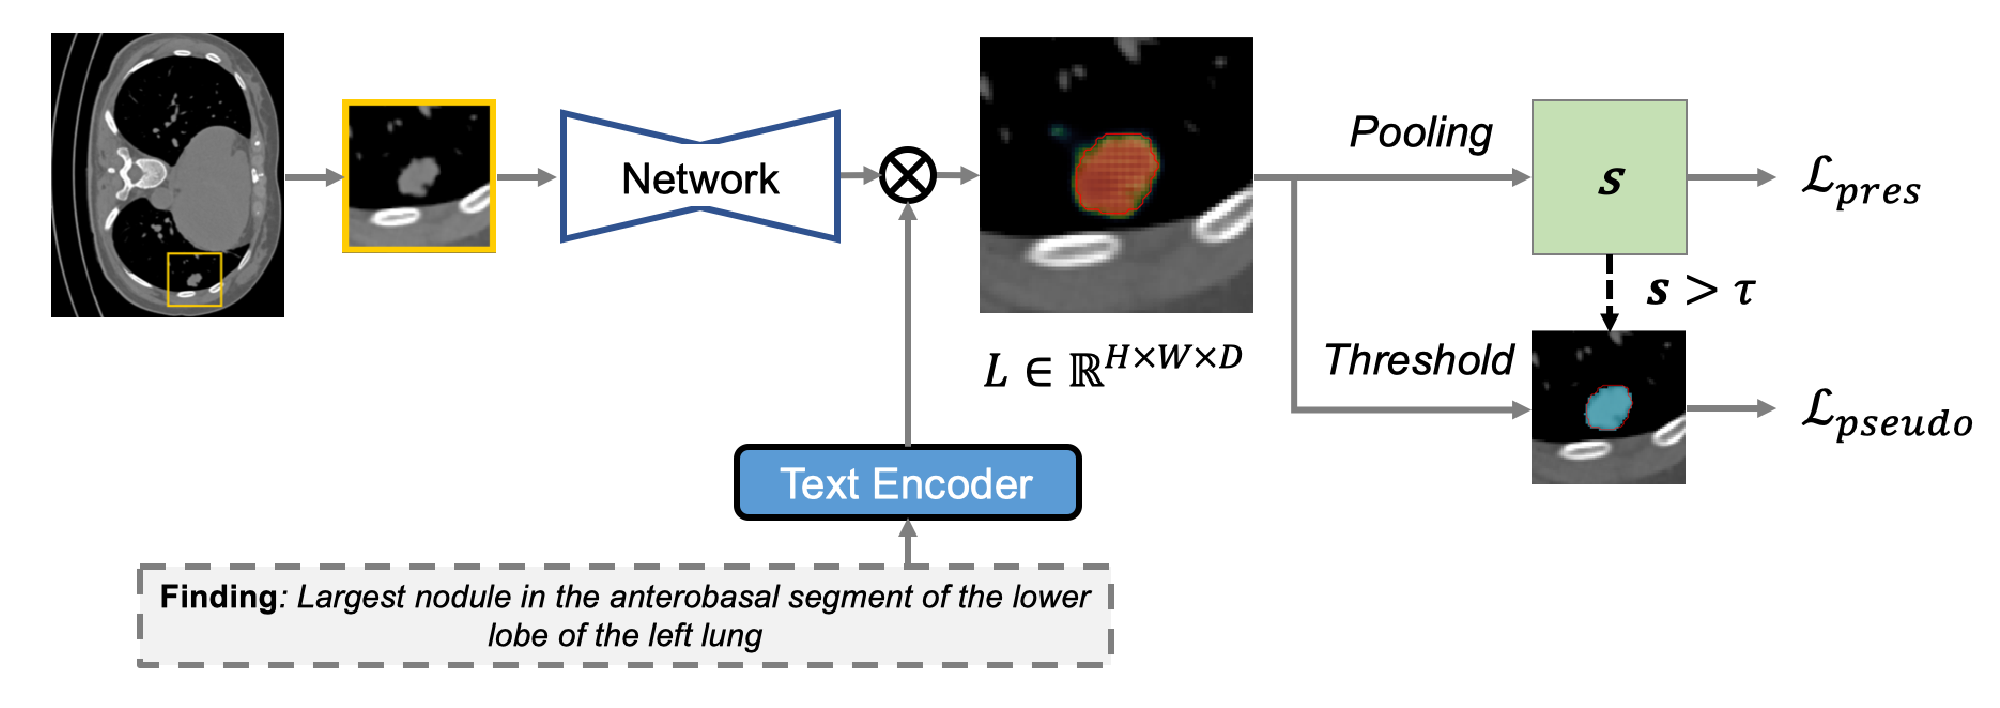
\includegraphics[width=\columnwidth]{figures/appendix/team4_semisupervised.pdf}
\caption{Team 4: semi-supervised training on CT-RATE (stage 2). Voxel logits for
the finding are pooled into a presence score trained against whether the finding
is present, and thresholded predictions of an EMA teacher serve as pseudo-masks.}
\label{fig:app-team4}
\end{figure}
